% !TEX TS-program = xelatex
% !TEX encoding = UTF-8 Unicode
\documentclass[11pt,a4paper]{article}
\usepackage{amsmath,amssymb}
\usepackage{empheq}
\usepackage[semibold]{ebgaramond}
\usepackage[cmintegrals,cmbraces]{newtxmath}
\usepackage{ebgaramond-maths}
\usepackage{bm}
\usepackage[OMLmathrm, OMLmathsfit, rmdefault=mdugm]{isomath}
\usepackage{tocbibind}

\makeatletter
  \DeclareSymbolFont{ntxletters}{OML}{ntxmi}{m}{it}
  \SetSymbolFont{ntxletters}{bold}{OML}{ntxmi}{b}{it}
  \re@DeclareMathSymbol{\leftharpoonup}{\mathrel}{ntxletters}{"28}
  \re@DeclareMathSymbol{\leftharpoondown}{\mathrel}{ntxletters}{"29}
  \re@DeclareMathSymbol{\rightharpoonup}{\mathrel}{ntxletters}{"2A}
  \re@DeclareMathSymbol{\rightharpoondown}{\mathrel}{ntxletters}{"2B}
  \re@DeclareMathSymbol{\triangleleft}{\mathbin}{ntxletters}{"2F}
  \re@DeclareMathSymbol{\triangleright}{\mathbin}{ntxletters}{"2E}
  \re@DeclareMathSymbol{\partial}{\mathord}{ntxletters}{"40}
  \re@DeclareMathSymbol{\flat}{\mathord}{ntxletters}{"5B}
  \re@DeclareMathSymbol{\natural}{\mathord}{ntxletters}{"5C}
  \re@DeclareMathSymbol{\star}{\mathbin}{ntxletters}{"3F}
  \re@DeclareMathSymbol{\smile}{\mathrel}{ntxletters}{"5E}
  \re@DeclareMathSymbol{\frown}{\mathrel}{ntxletters}{"5F}
  \re@DeclareMathSymbol{\sharp}{\mathord}{ntxletters}{"5D}
  \re@DeclareMathAccent{\vec}{\mathord}{ntxletters}{"7E}
\makeatother

\usepackage{array}
\usepackage{enumitem}
% to produce a comma between multiple footnotes / https://tex.stackexchange.com/questions/40072/incompatibility-between-footmisc-option-multiple-and-hyperref/62091#62091
\let\oldFootnote\footnote
\newcommand\nextToken\relax
\renewcommand\footnote[1]{%
    \oldFootnote{#1}\futurelet\nextToken\isFootnote}
\newcommand\isFootnote{%
    \ifx\footnote\nextToken\textsuperscript{,}\fi}

\defaultfontfeatures{Ligatures=TeX} % makes this a feature for all selected fonts
\usepackage{esint}
\usepackage{polyglossia}
\setmainlanguage{english}
\usepackage[text={18cm,26cm},centering]{geometry} % 
\usepackage{natbib}
\usepackage{graphicx}
\graphicspath{{./pics/}}
\usepackage{wrapfig}
\usepackage{mdframed}
\usepackage{lipsum}
\usepackage[usenames,dvipsnames,svgnames,table]{xcolor}
\usepackage{hyperref}
\usepackage{url}
\usepackage[export]{adjustbox}

\hypersetup{
  colorlinks,
  citecolor=bleuSU,
  linkcolor=bleuSU
}
\definecolor{bleuSU}{RGB}{26,39,101}

\usepackage[normalem]{ulem}
\makeatletter
\renewcommand*{\uuline}{%
  \bgroup
  \UL@setULdepth
  \markoverwith{%
    \lower\ULdepth\hbox{%
      \kern-.03em%
      \vtop{%
        \hrule width.2em%
        \kern 0.6pt % distance between the two underlines
        \hrule
      }%
      \kern-.03em%
    }%
  }%
  \ULon
}
\makeatother
\setlength{\ULdepth}{-2pt}  % distance from double underline to letter

\usepackage{environ}
\newtoggle{corrige}

\NewEnviron{answer}{%
  \iftoggle{corrige}
    {\begin{mdframed}\textbf{Answer: } \BODY\end{mdframed}}
    {}%
  }

\newcommand{\delS}{\delta S}
\newcommand{\delA}{\delta A}
\newcommand{\delh}{\delta h}
\newcommand{\delt}{\delta t}
\newcommand{\delz}{\delta z}
\newcommand{\delbx}{\delta \matrixsym x}
\newcommand{\lp}{\left(}
\newcommand{\rp}{\right)}
\newcommand{\itA}{\textit A}
\newcommand{\itB}{\textit B}
\newcommand{\dAB}{\mathcal D_{AB}}
\newcommand{\bA}{\matrixsym A}
\newcommand{\bff}{\matrixsym{f}}
\newcommand{\bF}{\matrixsym{F}}
\newcommand{\bj}{\matrixsym{j}}
\newcommand{\bJ}{\matrixsym J}
\newcommand{\bn}{\matrixsym{n}}
\newcommand{\bN}{\matrixsym N}
\newcommand{\bP}{\matrixsym{P}}
\newcommand{\br}{\matrixsym r}
\newcommand{\bt}{\matrixsym t}
\newcommand{\be}{\matrixsym e}
\newcommand{\bu}{\matrixsym u}
\newcommand{\bv}{\matrixsym v}
\newcommand{\bw}{\matrixsym w}
\newcommand{\bx}{\matrixsym x}
\newcommand{\pd}[2]{\frac{\partial #1}{\partial #2}}
\newcommand{\D}[2]{\frac{D #1}{D #2}}
\newcommand{\dd}[2]{\frac{\mathrm d #1}{\mathrm d #2}}
\newcommand{\dA}{\mathrm dA}
\newcommand{\dV}{\mathrm dV}
\newcommand{\dS}{\mathrm dS}
\newcommand{\prg}[1]{\paragraph{$\rhd$ #1}}
\newcommand{\alphaijkl}{\alpha_{ijkl}}
\newcommand{\Aijkl}{A_{ijkl}}
\newcommand{\delij}{\delta_{ij}}
\newcommand{\sigij}{\sigma_{ij}}
\newcommand{\sigji}{\sigma_{ji}}
\newcommand{\sigxy}{\sigma_{xy}}
\newcommand{\matL}{\mathcal L}
\newcommand{\matO}{\mathcal O}
\newcommand{\matS}{\mathcal S}
\newcommand{\kij}{k_{ij}}
\newcommand{\tensor}[1]{\smash{\uuline{#1}{}}}
\setlength{\parindent}{0pt} % remove indent
  
\begin{document}
\setlength{\unitlength}{1cm}
\noindent
\parbox{\textwidth}{
\textsc{
Sorbonne Université  
\hfill
Year 2021-2022
}
}
\parbox{\textwidth}{
\textsc{
Faculté des Sciences
\hfill
Physics of Fluids \& Nonlinear Physics
}
}

\begin{center}
\Large
\textbf{Hydrodynamics} \\ 
\textsl{Tutorial 1: fluid motion} \\[1ex]
\end{center}

%\vspace{5mm}
\section{Dimensional analysis}
\toggletrue{corrige}

\paragraph{$\rhd$ Imbibition.}  
\begin{figure}[ht]
    \centering
    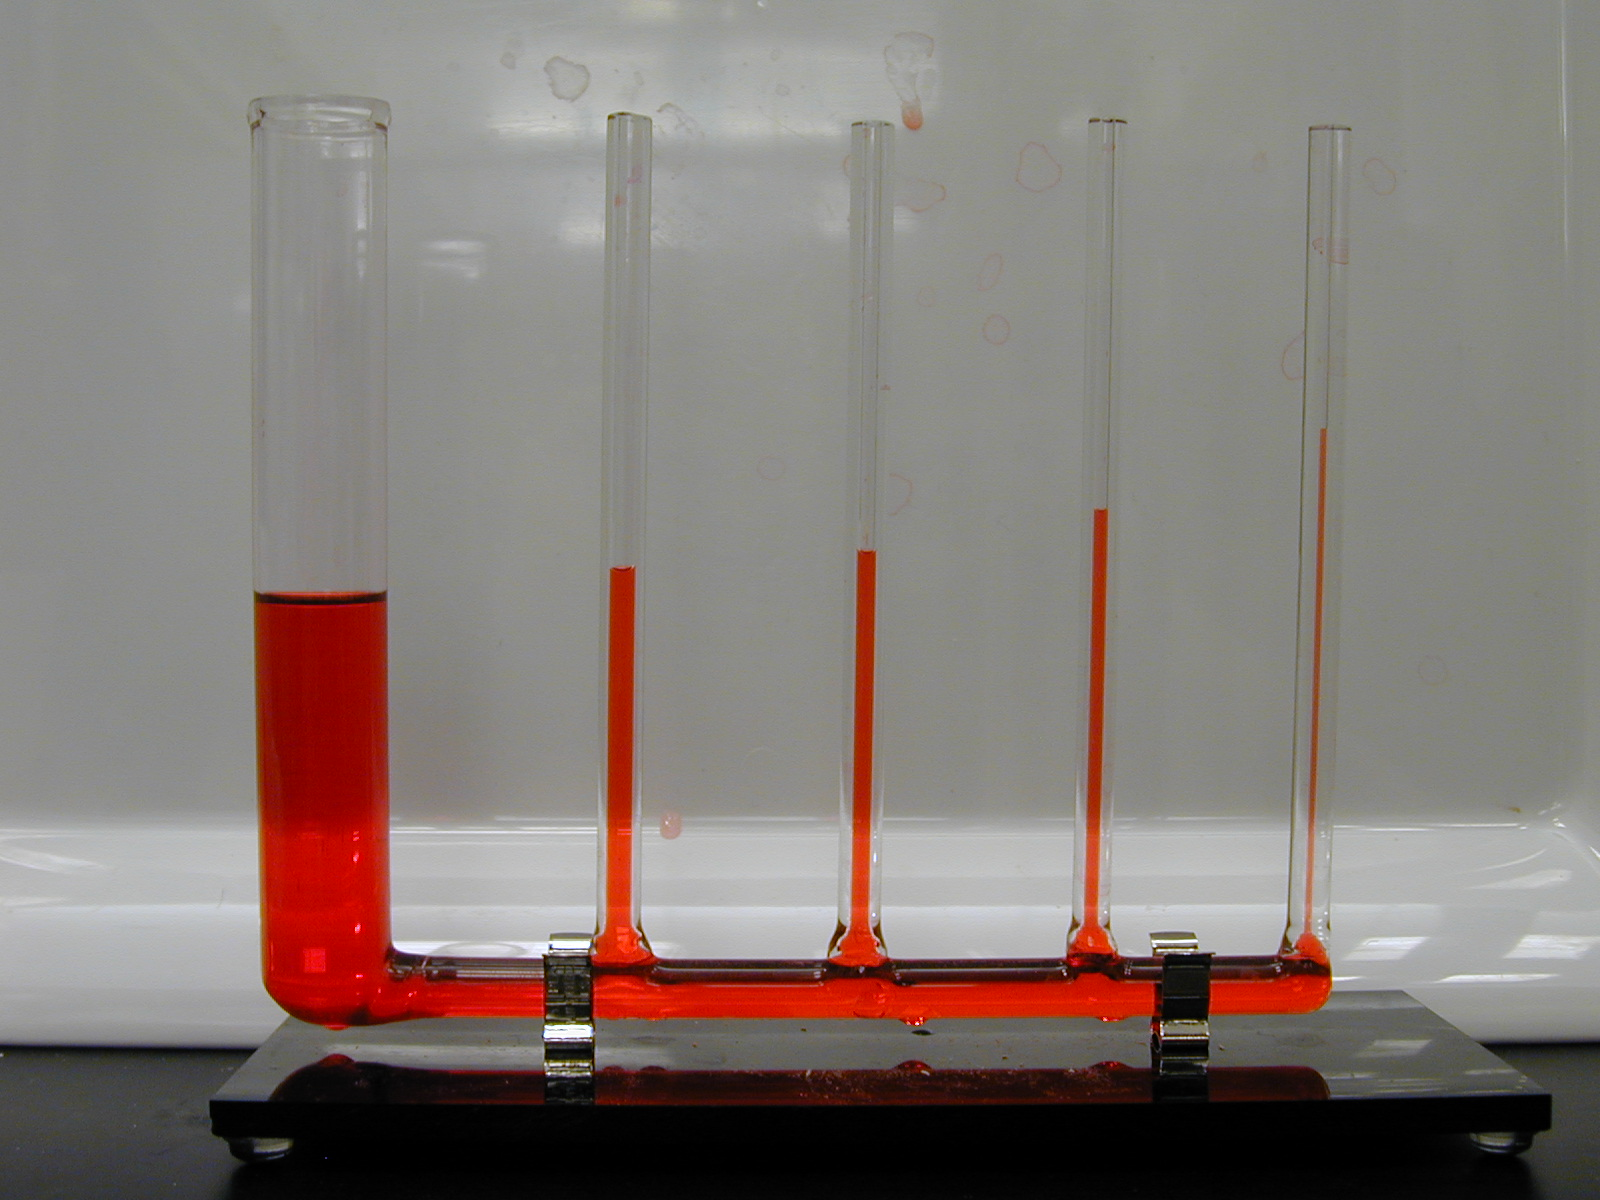
\includegraphics[height=5cm,valign=m]{capillaryrise.JPG}
    \hspace{1cm}
    \includegraphics[valign=m,page=2]{lucas.pdf}
    \caption{\textbf{Maximal ascension.} Left: the maximal height for capillary ascension depends on tube radius $R$. Right: maximal height $h$ observed for the capillary rise of ethanol in tubes of different radii $R$ (data from the authors).}
    \label{fig:jurin}
\end{figure}
A narrow capillary tube is brought into contact with a wetting liquid. The liquid spontaneously rises in the tube up to a height $h$ (figure~\ref{fig:jurin}). This height depends a priori on the \textit{surface tension} $\gamma$ ($[\gamma] = \mathsf{MT}^{-2}$), gravity $g$, density $\rho$ and on the tube radius $R$ :
\begin{equation}
h = f(\gamma, \rho, g, R)
\end{equation}
\begin{enumerate}
\item Using the characteristic scales $\rho$, $g$ and $R$, show that the previous functional relation can be rewritten as:
\begin{equation}
\mathrm \pi = \mathcal F(\mathrm \pi_1),
\end{equation}
where $\mathrm \pi$ corresponds to the nondimensional height (the observable), and $\mathrm\pi_1$ to the non-dimensional surface tension. Write the expression for $\mathrm\pi$ and $\mathrm\pi_1$ (that we will take proportional to $h$ and $\gamma$ respectively).
\begin{answer}
\begin{equation*}
\pi = \frac{h}{R} \quad \text{ and } \quad \pi_1 = \frac{\gamma}{\rho g R^2}
\end{equation*}
\end{answer}

\item Experiments and physical analysis show that $\mathcal F(x) = 2x$. What is the scaling law of $h$ with respect to $R$ ? Is it compatible with the experimental results reported~\ref{fig:jurin} ?
\begin{answer}
We have $h = \frac{2\gamma}{\rho g R}$ therefore $h \propto \frac{1}{R}$, compatible with the experimental results.
\end{answer}
\end{enumerate}

\paragraph{$\rhd$ Molecular diffusion.} A drop of dye is delicately deposited in a liquid. Due to constant molecular motion and collisions, the area expands by \textit{diffusion} -- a process whose efficiency is characterised with the diffusion coefficient $D$ (of dimension $[D] = \mathsf{L^2T^{-1}}$). 
\begin{enumerate}[resume]
\item Using dimensional analysis show that the dye drop spreads following a square root law at long times $R(t) \propto t^{1/2}$.
\begin{answer}
$h = a \sqrt{Dt}$
\end{answer}
\end{enumerate}
\paragraph{$\rhd$ Turbulent diffusion.} \textit{(from \citet{Eggers2015})}. We consider again the previous experiment but now the liquid is vigorously stirred, so as as to create turbulent motions stirring and mixing the dye. This process is a priori much more efficient than simple molecular diffusion, so that we neglect the latter in the following. The stirring intensity is characterised with $\varepsilon$, the energy quantity per unit time and mass in the liquid. 
\begin{enumerate}[resume]
\item what is the dimension of $\varepsilon$ ?
\begin{answer}
$[\varepsilon] = \mathsf{L}^2\mathsf{T}^{-3}$
\end{answer}

\item Show that the drop area now grows according to
\begin{equation}
R(t) = A \lp \varepsilon t^3\rp^{1/2},
\end{equation}
where $A$ is a dimensionless universal constant. This result is the signature of a process much more efficient than molecular diffusion, and known as \textit{Richardson's law} \citep{Richardson1926,Eggers2015}.
\end{enumerate}


\section{Starting plane shear flow}
\begin{figure}[h]
\begin{center}
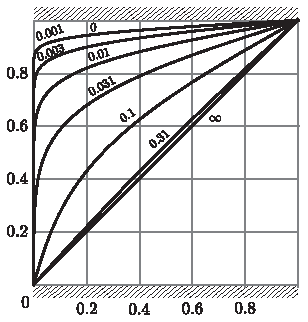
\includegraphics{transient_couette.pdf}
\end{center}
\caption{\textbf{Transient of a Couette flow}. Several successive velocity profiles are shown here as a function of the nondimensional time $\bar t = \nu t / h^2$.}
\end{figure}

\noindent We are interested here in the setting up of a fluid flowing in between two parallel plates of infinite extension when one of them is suddenly set into motion \citep{Batchelor1967,Ockendon1995}. The plates are separated with a distance~$h$. At $t=0$ the upper plate is abruptly set into motion at velocity $\matrixsym U = (U,0,0)$. The fluid, at rest until that moment, starts progressively to move due to momentum diffusion until it reaches the Couette steady-state. Note also that there is no imposed pressure gradient and that momentum diffusion is the only cause for fluid motion. The dynamic viscosity of the fluid is noted~$\mu$, the kinematic viscosity $\nu$ and we neglect the action of gravity. We will consider an translation-invariant evolution along the two directions parallel to the plates (this amounts to consider a \textbf{parallel} flow) and we will also suppose that the flow is \textbf{incompressible}\footnote{Over very short times of the order $h/c$ with $c$ the sound celerity in the fluid, this hypothesis can be invalidated. But we can put figures to get an idea by taking e.g. water as a working fluid ($c\simeq 1500 \text{m}\cdot\text{s}^{-1}$) and $h = 1 \text{cm}$ as the distance between the plates. The acoustic timescale. is then of the order of 7 $\mu$s to be compared with the diffusive timescale exceeding a minute (7 orders of magnitude apart!). Moreover it is quite possible that in the experimental setup the starting of the plate cannot be considered impulsive over the acoustic timescale.}.
\begin{enumerate}
    \item Propose an estimation of the order of magnitude of the viscous shear stress exerted on one of the plate in the steady limit, along with an estimation of the typical transient timescale.
\begin{answer}
The viscous shear stress $\tau$ corresponds to the product between viscosity and the wall shear, that we can estimate here with $U/h$.
 We therefore get;
 $$
 \tau \sim \mu \frac{U}{h}.
 $$
The typical transient timescale is a \textbf{diffusive} timescale (vertical diffusion of horizontal momentum) and is $h^2/\nu$.
\end{answer}
    \item Write down the equations expressing mass and momentum conservation (using scalar projections), along with the boundary conditions and the initial condition of the problem. Beware of neglecting the unsteady terms.
     \item Nondimensionalise the equations using the natural scales of the problem by setting $y = h \bar y, u = U \bar u$ and $t = h^2 \bar t / \nu$. 
    \begin{answer}
    We get :
    $$
    \pd{\bar u}{\bar t} = \frac{\partial^2 \bar u}{\partial \bar y^2},
    $$
    associated to 
    \begin{empheq}[left=\empheqlbrace]{alignat=2}
&\text{bottom plate no-slip condition} :\qquad &  \bar u(0,\bar t) = 0,\nonumber \\
&\text{upper plate no-slip condition} :\qquad & \bar u(1,\bar t) = 1,\nonumber\\
&\text{initial condition} :\qquad & \bar u(\bar y,0) = 0.\nonumber
\end{empheq}
    \end{answer}
    \item In the steady limit, determine the flow profile $\bar u_\text{couette}(\bar y)$ along with its gradient, and deduce the dimensioned value of the wall shear stress both at the bottom and at the top plate. 
\end{enumerate}
\noindent We now seek to describe the onset of this flow with a solution of the form:
\begin{equation}
\bar u(\bar y,\bar t) = \bar u_\text{couette}(\bar y) + \bar u_\text{unst}(\bar y,\bar t)
\label{eq:profile}
\end{equation}
\begin{enumerate}[resume]
    \item Injecting the profile~(\ref{eq:profile}) in the equations for motion, obtain a new set of equations and boundary conditions for $\bar u_\text{unst}(\bar y,\bar t)$. What is the initial condition for  $\bar u_\text{unst}(\bar y,0)$ ? 
    \begin{answer}
    Same equation (linearity). Homogeneous BC and $\bar u_\text{unst}(\bar y,0) = -\bar y$.
    \end{answer}
    \item We look for a solution by using the variable separation technique, i.e. we pose $\bar u_\text{unst}(\bar y,\bar t) = f(\bar y)g(\bar t)$. Obtain the equations governing $f(\bar y)$ and $g(\bar t)$ along with the general form of the solutions.
    \item Show that the application of the boundary conditions imposes a quantisation condition on the solutions. Deduce the form of the velocity profile as a Fourier series whose coefficients are yet to be determined.
    \item Demonstrate the orthogonality relation:
    $$
     \int_0^1 \sin(n \pi x) \sin(m \pi x) \, \mathrm dx = \begin{cases*} 0 & if  $n \neq m$ \\ \frac{1}{2} & if $n = m$ \end{cases*}
    $$
    \item Exploit the orthogonality relation so as to determine the flow transient, then show that the dimensioned expression for the velocity field is
    \begin{equation}
    u(y,t) = \frac{U y}{h} + \sum_{n=0}^\infty \frac{2U}{n\mathrm\pi} \lp-1\rp^n \sin\lp\frac{n\mathrm\pi y}{h}\rp e^{-\frac{n^2 \mathrm\pi^2}{h^2}\nu t}
    \end{equation}
\item What is the asymptotic solution? What is the first correction for long times?
\end{enumerate}
\subsection*{Short project}
Design a numerical code to solve this problem. Compare the numerical solution with the (truncated) series. How many terms are required? Does this number change with time? Represent the evolution of the bottom wall shear stress with time and compare it with the truncated series. Same question but for the \textit{upper} plate. Why does it fail at short times? 
%    \item Calculer l'évolution de la contrainte de cisaillement sur la plaque du haut et sur la plaque du bas. 
%    \item Tracer numériquement le champ de vitesse et l'évolution de la contrainte en tronquant la série. Combien de termes est-il nécessaire de garder pour avoir une représentation convergée ? 

\section{Poiseuille flow in a tube of arbitrary shape}
\noindent A fluid flows in a tube of uniform section (not necessarily circular) under the action of a constant pressure gradient $-\frac{\partial p}{\partial x}$. We suppose that the flow is fully established (no $x$ dependency) and parallel ($v = w = 0$). For given tube section $A$ and pressure gradient, we look for the tube geometry that minimises the total viscous force exerted on the wall \citep{Ockendon1995}.
\begin{figure}[h]
\begin{center}
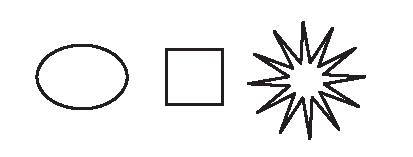
\includegraphics[width=9cm]{poiseuille_shapes.pdf}
\end{center}
\caption{A family of tubes of constant section, but with different shapes.}
\end{figure}

\begin{enumerate}
\item Show the relation:
$$
\mu\left( \frac{\partial^2 u}{\partial y^2} + \frac{\partial^2 u}{\partial z^2} \right) = c.
$$
What is the the meaning of $c$ here?
\item Show that the total viscous force exerted on the wall takes the following expression:
$$
\oiint_{\partial D} \mu \frac{\partial u}{\partial n} \, \mathrm dS.
$$
%    $$
%   \sigma_{xj} (0,n_y,n_z)=\sigma_{xy} n_y + \sigma_{xz} n_z = \mu ( u_{x,y} ) n_y + \mu u_{x,z} n_z = \mu u_{,n}
%    $$
\item On using Green's formulae:
$$
\iiint_V \Psi \nabla^2 \varphi\,\mathrm dV = - \iiint_V \nabla \Psi \cdot \nabla \varphi\,\mathrm dV + \oiint_{\partial V} \Psi \frac{\partial \varphi}{\partial n} \, \mathrm dS,
$$
Answer the question.
\item Show that we could retrieve this result in a blink by conducting a force balance on a fluid portion.
\begin{answer}
The viscous force per unit length is $\pd{p}{x} A$, and does not depend on the tube shape. This result might be surprising at first because we could have expected a more ``dented'' tube, or a tube exposing a higher contact surface, to bear a higher viscous force.
But actually if we consider a fluid portion of length $L$ flowing steadily, we see that the driving force $-\pd{p}{x} A L$ has to be balanced with a resistive force $\tau L$ ($\tau$ being the viscous stress integrated on a section). Hence the result.
\end{answer}

\end{enumerate}
\bibliographystyle{jfm}
\bibliography{biblio_tuto}
\end{document}